{	% Background Image
	\usebackgroundtemplate{
	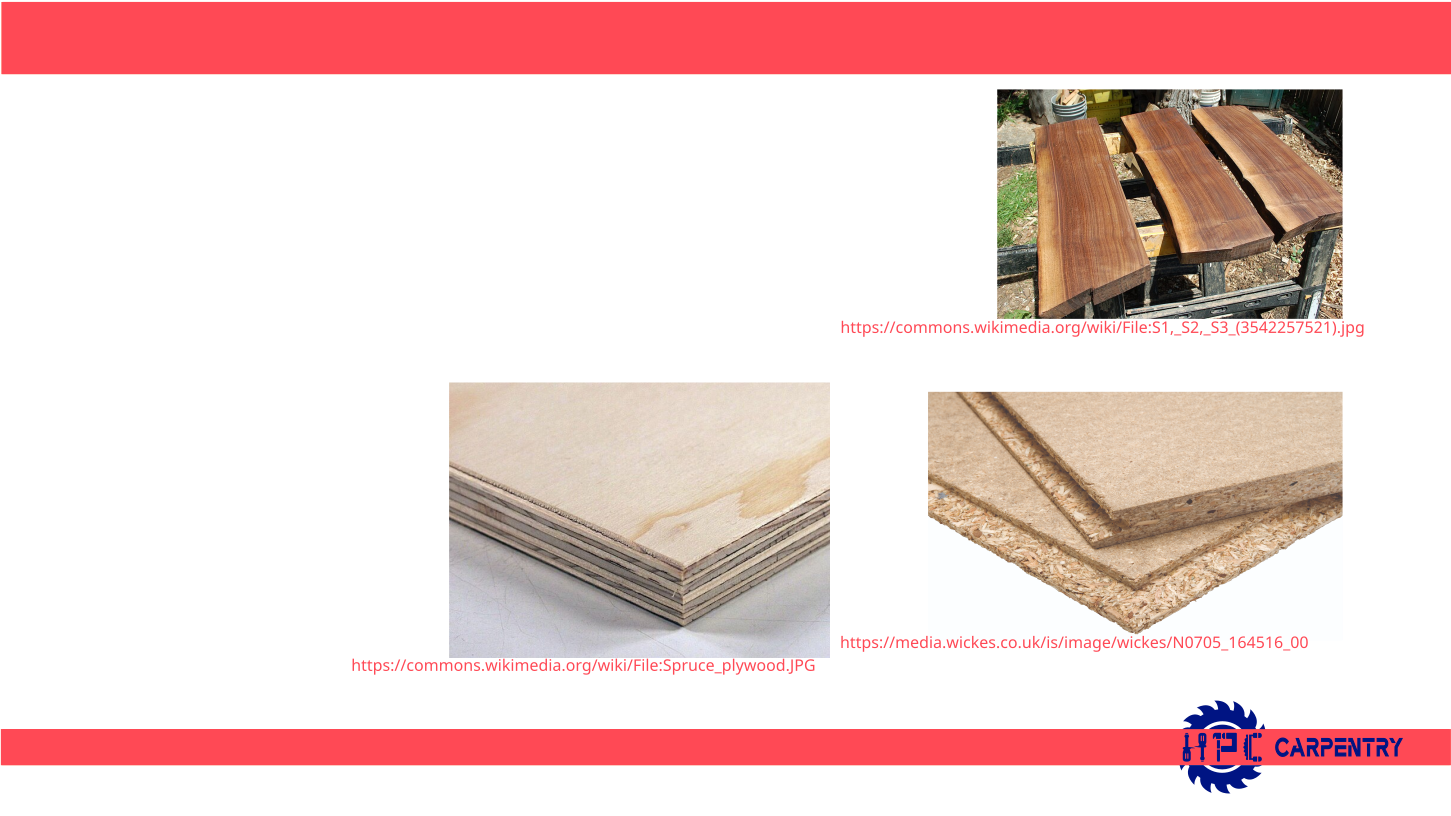
\includegraphics[width=\paperwidth]{images/choices.png}
}
\begin{frame}{HPC means we have choices}
	\note[item]{HPC could potentially stand for hardwood, plywood and chip board}
	\begin{enumerate}
		\item \textbf{H}ardwood
		\item \textbf{P}lywood
		\item \textbf{C}hip board
	\end{enumerate}

\note{}
\end{frame}
}

{	% Background Image	\note<2>[item]{Say something to the audience!}
	\usebackgroundtemplate{
	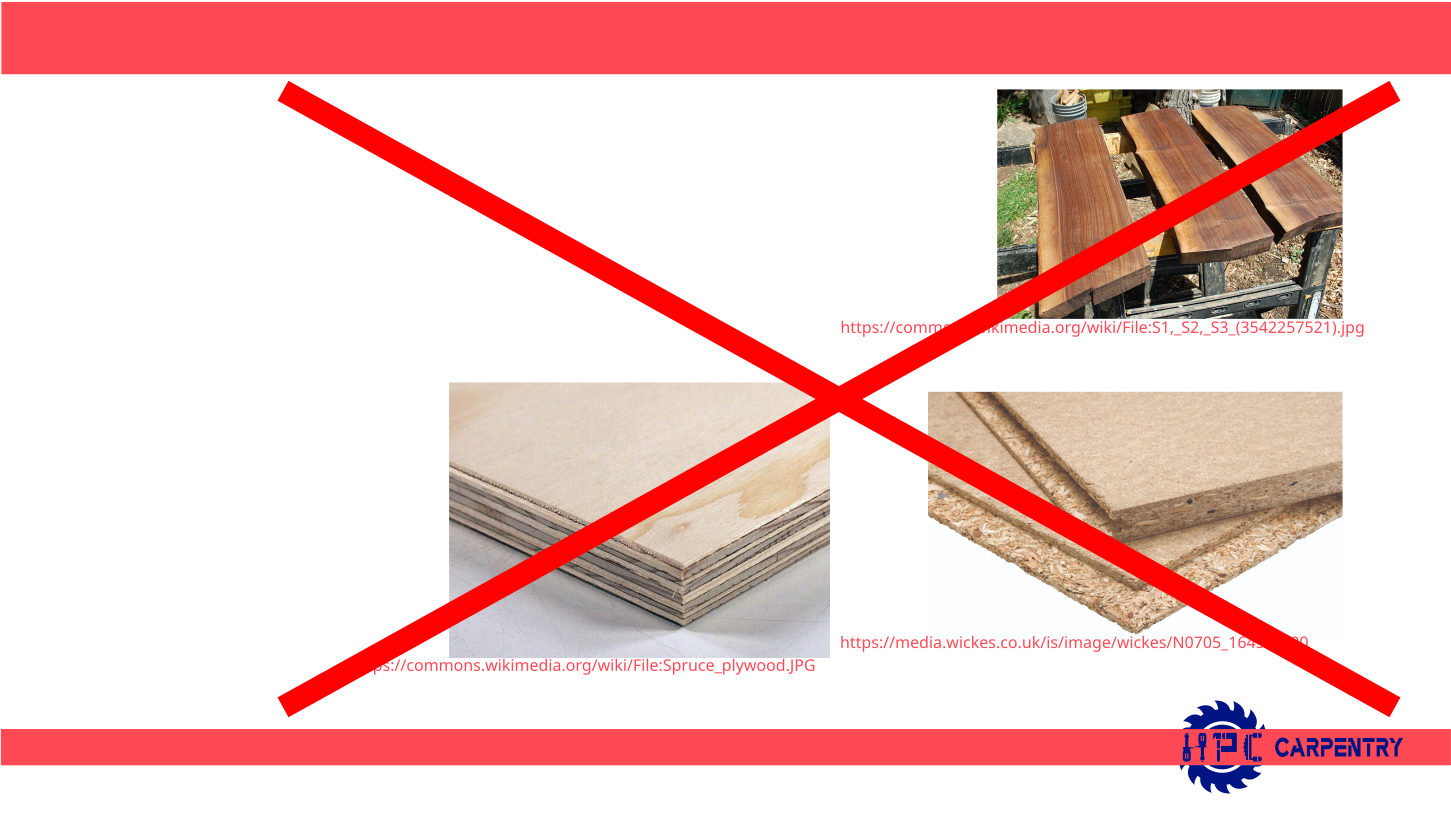
\includegraphics[width=\paperwidth]{images/Xchoices.png}
}
\begin{frame}{But that has nothing to do with anything ...}
	\begin{enumerate}
		\item \textbf{H}ardwood
		\item \textbf{P}lywood
		\item \textbf{C}hip board
	\end{enumerate}
	
	\note[item]{But, this type of HPC actually has nothing to do with what I'm about to tell you but I thought I'd mention it anyway.}
\end{frame}
}
